\chapter{Initial Evaluation}\label{C:init_eval}

\section{Initial Experimental Setup at Project Start}
Given that the express purpose of the project is the development of a new version of instrumentation, the first step is an examination of the prior system. This is to identify how it falls short and to determine the areas that the project will focus on.

The experimental method concerns depositing a liquid droplet upon a heated substrate. The data of note is the temperature evolution of the substrate directly under the drop, as well as image data capturing the point of impact and how the droplet changes over the cause of the evaporation.

\begin{figure}[h]
    \begin{center}
        \includegraphics[width=.4\textwidth]{example-image}
        \caption{Current Experimental Setup (labelled/annotated to be included) a:diagram b:syringe stage}
        \label{fig:prior_exp}
    \end{center}
\end{figure}
The prior system uses an optical breadboard and micrometer adjustable stages as mounting platforms and positional control.
A central stage holds the substrate stack, consisting of a aluminium heat-spreader, Peltier heater, and metallic substrate (copper, stainless steel, etc) with internally mounted thermocouple.
To capture the image data, a pair of manual focus cameras are positioned/suspended in profile and top down view and are controlled via a USB connection. The thermocouple is sampled with LabVIEW via a USB DaQ.
Dispensing the droplet itself is done by hand using a syringe mounted to another optical stage [\ref{fig:prior_exp}:b] with XYZ+R controls. It is rotated above the substrate and pressed to dispense a drop.

This would be perfectly fine, however the results this manual process yields had a level of inconsistency. Thus motivating the design of a new system to control for a the experiments variation.

\newpage
\section{Repeatability and Reliability}
To identify more precisely the drawbacks in the performance of the prior setup and inform the requirements of the project, previously collected data was first analysed.

The data was taken from a series of five droplet runs, and was analysed to quantify the systems repeatability and reliability and to compare the affect of the drop morphology and position with the resulting temperature evolution.

\begin{figure}[h]
    \begin{center}
        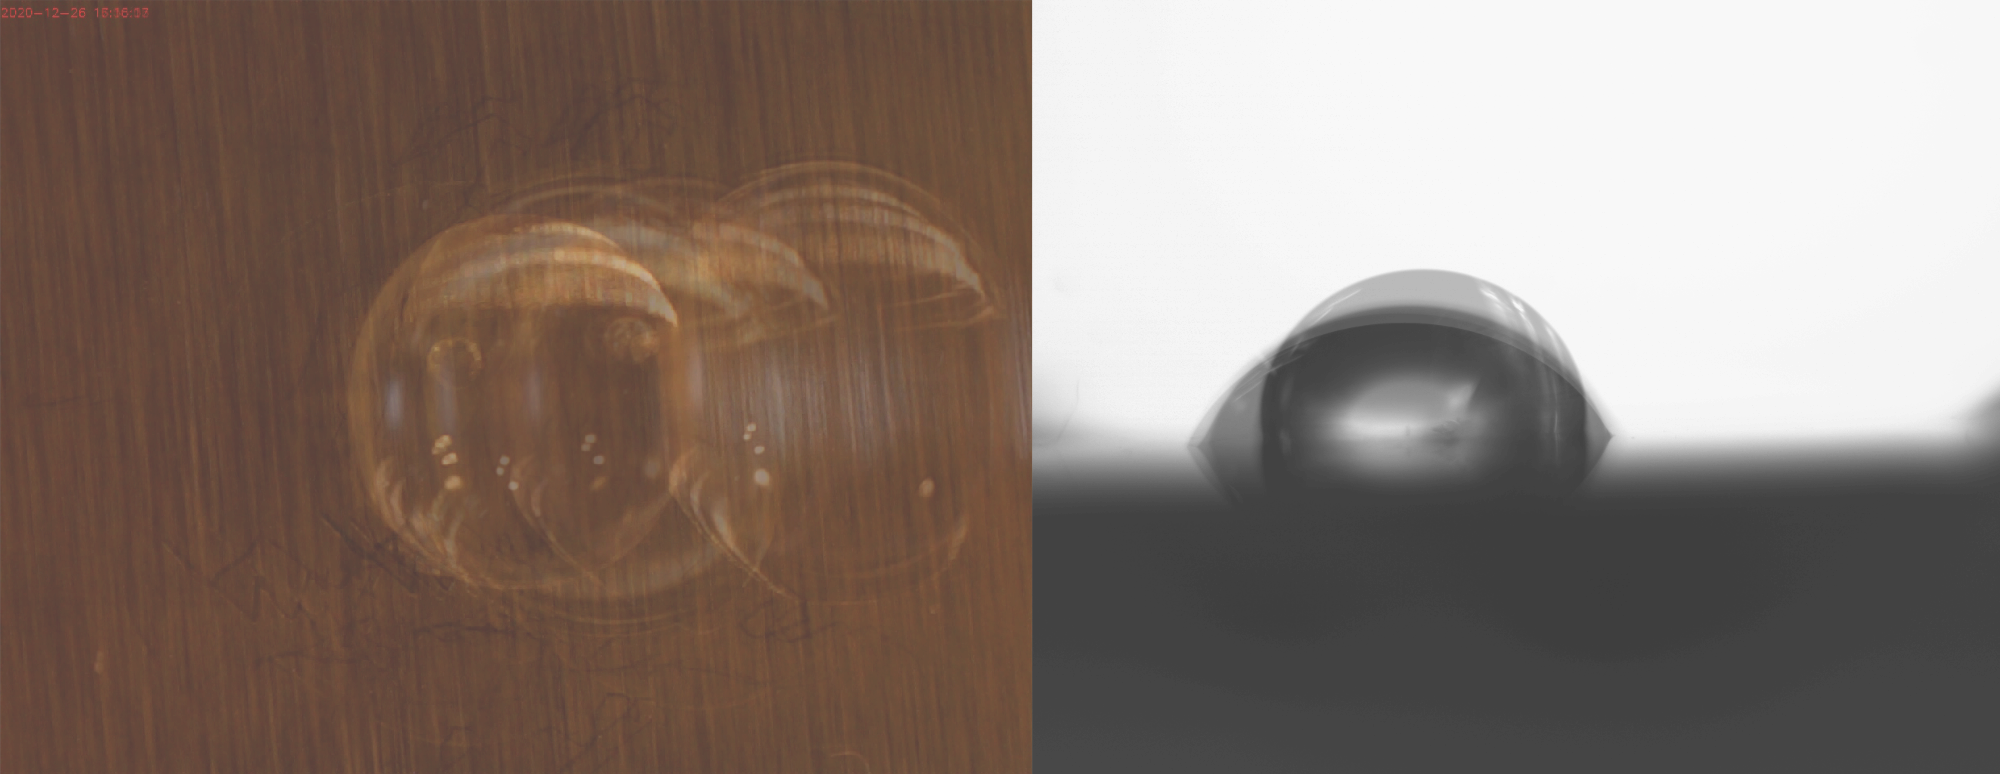
\includegraphics[width=.4\textwidth]{img/droplets_2018.png}
        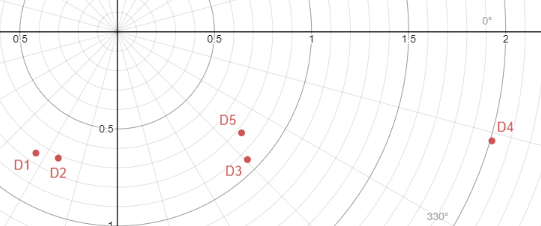
\includegraphics[width=.4\textwidth]{img/drop_pos_2018.png}
    \end{center}
\end{figure}

First analysis is the image data. The substrate itself has a mark to represent the position of the thermocouple, this is used as a the main reference to quantify the droplet position. Reference images set calibration at 120.14 pixels/mm and 109.2 pixels/mm for the top down and profile cameras respectively, and was used to measure the droplet centre offset and angle (from reference point) as well as the height, width and contact angles of the droplet on the substrate.

Seen above, the quite substantial positional variation between the runs. Ranging [0.71:2.01]mm offset and [-16:-123]$^\circ$ angle.


\begin{equation}
    \frac{1}{6}\pi h(3a^2 + h^2)
    : a \equiv \mathrm{half \; width}, \; h \equiv \mathrm{height}
    \label{equ:vol}
\end{equation}
From the data extracted from the profile camera (height, width, contact angle) the volume of the droplets could be estimated. The method chosen was of the represent the droplet as a spherical cap and use the above equation \ref{equ:vol} to compute it.

\begin{figure}[h]
    \begin{center}
        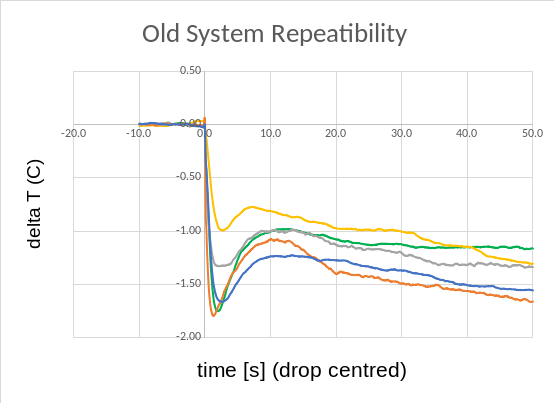
\includegraphics[width=.4\textwidth]{img/drop_temps_2018.png}
        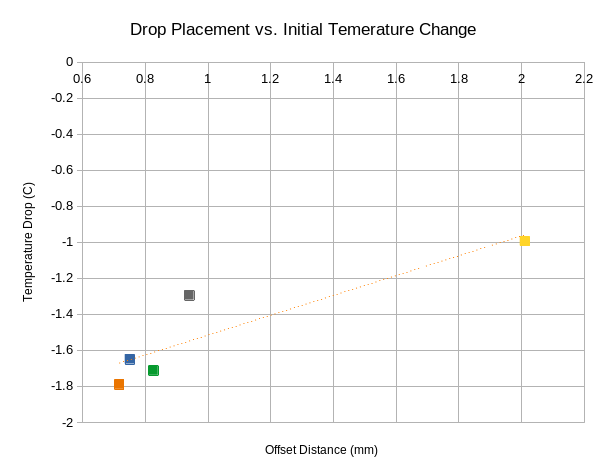
\includegraphics[width=.4\textwidth]{img/2018_pos_temp_trend.png}
    \end{center}
\end{figure}

\begin{table}[h]
    \centering
    \begin{tabular}{|l|l|l|}
        \hline
        \textit{\textbf{Droplet}}                          & \textit{Offset(mm)} & \textit{Volume(uL)} \\ \hline
        \cellcolor[HTML]{9698ED}1                          & 0.7506              & 16.55               \\ \hline
        \cellcolor[HTML]{E9AD3F}2                          & 0.7164              & 17.91               \\ \hline
        \cellcolor[HTML]{C0C0C0}3                          & 0.9402              & 17.89               \\ \hline
        \cellcolor[HTML]{FFFC9E}4                          & 2.0104              & 17.57               \\ \hline
        \cellcolor[HTML]{79CD5D}5                          & 0.8258              & 16.21               \\ \hline
        \cellcolor[HTML]{FFFFFF}\textbf{\textit{Variance}} & \textit{0.2964}     & \textit{0.6288}     \\ \hline
    \end{tabular}
\end{table}

\section{Summary}
\begin{table}[h]
    \centering
    \begin{tabular}{|l|l|l|}
        \hline
        \textbf{Effector} & \textbf{Likelihood} & \textbf{Effect Strength} \\ \hline
        Position          & HIGH                & HIGH                     \\ \hline
        Volume            & MODERATE            & HIGH                     \\ \hline
        Contact angle*    & MODERATE            & HIGH                     \\ \hline
        Humidity          & LOW                 & HIGH                     \\ \hline
        Temperature       & LOW                 & HIGH                     \\ \hline
        Pressure          & MODERATE            & MODERATE                 \\ \hline
    \end{tabular}
\end{table}
\textit{\small{*Contact angle is more a function of the surface cleaning of the substrate, and is only representative of the surface area of contact with the substrate}} \\

//TODO rewrite in prog
The focus of the project is now twofold. Firstly on the automation of the process to allow for faster, pre-programmed runs to be carried out easier, and secondly to improve on the repeatability and reliability of the results by controlling the procedural factors of the experiment.

An electronic pipette will be used to dispense a precise volume, and motorised stages will be used to provide pre-programmed, repeatable motion. The environmental factors however are not to be ignored, though controlling them is outside of the scope of this project. They will, however, be monitored, and this project will implement data collection of temperature, atmospheric pressure and humidity so these factors can be correlated to any remaining variation in data.